\documentclass{beamer}
\usepackage[comma,numbers,compress,square]{natbib}
\usepackage{listings}
\usetheme{polymtl}
\title{BittyBuzz}
\subtitle{Buzz for microcontrollers}
\author{Emir K. Belhaddad, Anthony Dentinger}
\date{\today}

\graphicspath{{resources/}}


% ========================================
% =               DOCUMENT               =
% ========================================

\begin{document}
	
	% ----------------------------------------
	% -                 CODE                 -
	% ----------------------------------------
	% Doing it this way is the only way I found to insert code blocks
	
	\defverbatim[colored]\buzzCClosure{
		\begin{lstlisting}[language=C,linewidth=5cm,basicstyle=\ttfamily\scriptsize,keywordstyle=\color{blue}]
int buzz_c_closure(buzzvm_t vm) {
  // Error if not passed 1 param.
  buzzvm_lnum_assert(vm, 1);

  // Take int value of param.
  buzzvm_lload(vm, 1);
  int16_t param1 =
    buzzvm_stack_at(vm, 1)->i.value;
  buzzvm_pop(vm);
	
  buzzobj_t result;
  // Compute result...

  buzzvm_push(result);
  return buzzvm_ret1(vm);
}
		\end{lstlisting}
	}
	
	\defverbatim[colored]\bittybuzzCClosure{
		\begin{lstlisting}[language=C,basicstyle=\ttfamily\tiny,keywordstyle=\color{blue}]
void bbz_c_closure() {
  // Error if not passed 1 param.
  bbzvm_assert_lnum(1);

  // Take int value of param.
  int16_t param1 =
    bbzheap_obj_at(
      bbzvm_locals_at(1))->i.value;


  bbzheap_idx_t result;
  // Compute result...

  bbzvm_push(result);
  bbzvm_ret1();
}
		\end{lstlisting}
	}

	% ----------------------------------------
	% -                SLIDES                -
	% ----------------------------------------
	
	\begin{frame}
		\titlepage
	\end{frame}
	\begin{frame}
		\frametitle{Introduction}
		\begin{itemize}
			\item Buzz: \textbf{Description of collective swarm behavior} with both top-down and bottom-up approaches \cite{buzz_arxiv}. Details of information propagation are hidden.
			\item Swarm intelligence and behavior require large numbers of robots with limited resources $\Rightarrow$ result must be achieved with the \textbf{cheapest robots possible}.
		\end{itemize}

		\centering \Large
		\textbf{How cheap can Buzz go?}
	\end{frame}
	\begin{frame}
		\frametitle{Introduction}
		\textbf{BittyBuzz}: Reimplementation of Buzz for microcontrollers. Designed for very cheap robots with extreme resource constraints.\\
		Currently, only implementation is for Kilobots, inexpensive robots designed to swarm in the thousands \cite{kilobot_paper}.
	\end{frame}
	\begin{frame}
		\frametitle{Outline}
		\tableofcontents
	\end{frame}
	\begin{frame}
		\section{Meeting Constraints}
		\begin{table}
			\begin{tabular}{l|c|c}
				& Khepera IV        & Kilobot\\
				\hline
				Processor         & 32-bits @ 800 MHz & 8-bits @ 8 MHz\\
				Flash             & 512 MB (+ 4 GB)   & 32 KB\\
				RAM               & 512 MB            & 2 KB\\
				Payload bandwidth & $\sim$ 1 MB/s \footnote{Assuming CCK modulation scheme} \cite{khepera_wifi}  & 350-450 B/s\\
				Packet drops      & None with TCP/IP  & $\approx$ 50\%
			\end{tabular}
			\caption{
				\label{table:khepera kilobot comparison}Table \ref{table:khepera kilobot comparison}: Resource comparison between the Khepera IV and Kilobot robots \cite{khepera_specs}}
		\end{table}
	\end{frame}
	\begin{frame}
		\section{$BittyBuzz \approx Buzz$}
		Differences between Buzz and BittyBuzz are minimal. Nonetheless, \textbf{what differences have resulted from these limitations?}\\
		\[Buzz - BittyBuzz =~?\]
		Theorem (accepted):
		\begin{align}
		\begin{split}
		Buzz - BittyBuzz = ~&\Delta Architecture + \Delta (Buzz~features)\\
		+ &\Delta (Closure~definitions) + (small~details)
		\end{split}
		\end{align}
	\end{frame}
	\begin{frame}
		\subsection{Architecture}
		\frametitle{Architecture}
		Microcontrollers with no standardized OS $\Rightarrow$ existance of platform-dependant operations.\\
		Out of the box, BittyBuzz thus has \textbf{two layers of implementation}:
		\begin{itemize}
			\item Higher-level "core" layer for \textbf{platform-independant operations} (VM bytecode execution, definition of \texttt{swarm}, \texttt{stigmergy}, ...).
			\item Thin, lower-level robot layer for \textbf{platform-dependant operations} (fetching bytecode, displaying errors, sending and receiving packets, ...). Must be implemented for each robot.
		\end{itemize}
	\end{frame}
	\begin{frame}
		\subsection{Buzz features}
		\frametitle{Buzz features}
		Consistency with Buzz has been a key factor to the development choices, however \textbf{some features still have limitations}. Examples:
		\begin{itemize}
			\item Only one \texttt{stigmergy} allowed ;
			\item \texttt{stigmergy} topic must be a string (currently, but can be overcome) ;
			\item \texttt{swarm} IDs range from 0 to 7.
		\end{itemize}
	\end{frame}
	\begin{frame}
		\subsection{Closure definitions}
		\frametitle{Closure definitions}
		Buzz C closures allow a user to call a C function from the Buzz side. Making them in BittyBuzz is also very similar.\\
		~\\
		\begin{figure}
			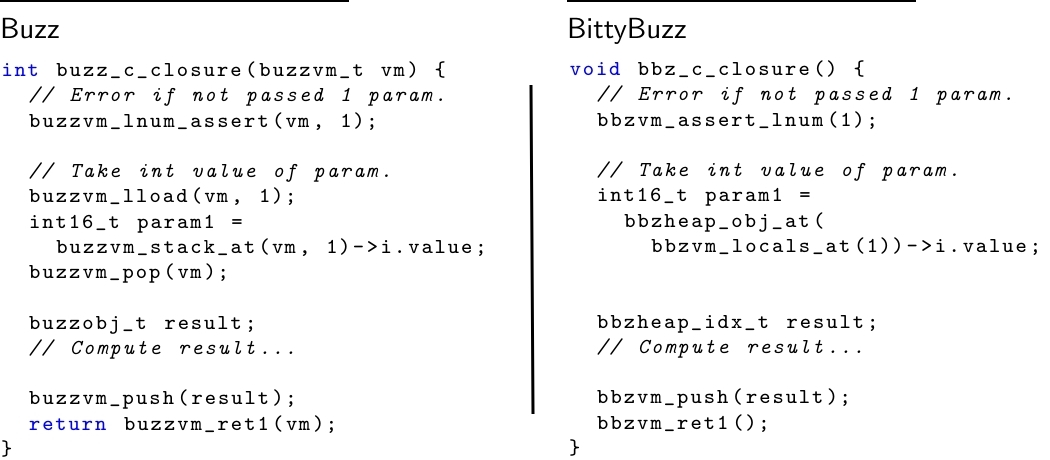
\includegraphics[width=1\textwidth]{ClosureDefinitions}
			\caption{\label{figure:C Closures}Fig. \ref{figure:C Closures}: C Closures in Buzz vs. BittyBuzz}
		\end{figure}
	\end{frame}
	\begin{frame}
		\section{Project results}
		Lorem ipsum dolor sit amet etc.
	\end{frame}
	\begin{frame}
		\section{}
		\frametitle{Concluding words}
		Lorem ipsum dolor sit amet etc.
	\end{frame}
	\begin{frame}
		\section{Future work}
		So that's it?\\
		No. There is still more work to be done for BittyBuzz:
		\begin{itemize}
			\item Implementation of \textbf{BittyBuzz for zooids}.
			\item Keep BittyBuzz up to date with new Buzz features.
			\item General improvements.
			\item Conduct \textbf{research projects using BittyBuzz}.
		\end{itemize}
		~\\
		\begin{quote}
			When you're finished changing, you're finished. -- Benjamin Franklin
		\end{quote}
	\end{frame}
	\begin{frame}
		\frametitle[allowframebreaks]{References}
		\bibliographystyle{IEEEtran}
		\bibliography{refs}
	\end{frame}
\end{document}
